%% %%=================================================================
%% %% <UTF-8>
%% %% 北航学位论文模板使用样例
%% %% 请将以下文件与此LaTeX文件放在同一目录中.
%% %%-----------
%% %% buaa.cls                  : LaTeX宏模板文件
%% %% bst/GBT7714-2005.bst      : 国标参考文献BibTeX样式文件2005(https://github.com/Haixing-Hu/GBT7714-2005-BibTeX-Style)
%% %% bst/GBT7714-2015.bst      : 国标参考文献BibTeX样式文件2015(https://github.com/zepinglee/gbt7714-bibtex-style)
%% %% pic/logo-buaa.eps         : 论文封皮北航字样
%% %% pic/head-professional.eps : 论文封皮专业硕士学位论文标题(华文行楷字体替代解决方案)
%% %% tex/*.tex                 : 本模板样例中的独立章节
%% %%-----------
%% %% 请统一使用UTF-8编码.
%% %%=================================================================

%=================================================================
% buaa基于ctexbook模板
% 论文样式参考自《研究生手册--二〇二〇年七月》
%======================
% 模板导入:
% \documentclass[thesis,permission,printtype,ostype,<ctexbookoptions>]{buaa}
%======================
%--------------------
% III.打印设置(printtype)
%--------------------
% a.单面打印(oneside)[缺省值]
% b.双面打印(twoside)
%--------------------
% IV.系统类型(ostype)
%--------------------
% a.win(oneside)[缺省值]
% b.linux (linux)
% c.mac (mac)
%--------------------
% V.ctexbook设置选项(<ctexbookoptions>)
%--------------------
% ...
%======================
% 其他说明:
% 1. Mac系统请使用mac选项,并使用XeLaTeX编译。
% 2. 可加入额外ctexbook文档类的选项,其将会被传递给ctexbook。
%    例如:\documentclass[fontset=founder]{buaa}
% 3. CTeX在Linux下默认使用Fandol字体,为避免某些生僻字无法显示,在系统已安装方正
%    字体的前提下可通过fontset=founder选项常用方正字体。
%=================================================================

% !TeX program = xelatex

\documentclass[oneside,win]{buaa}

%=================================================================
% 开启/关闭引用编号颜色:参考文献,公式,图,表,算法 等……
\refcolor{on}   % 开启: on[默认]; 关闭: off;
% 摘要和正文从右侧页开始
\beginright{off} % 开启: on[默认]; 关闭: off;

%=================================================================
% buaa模板已内嵌以下LaTeX工具包:
%--------------------
% ifthen, etoolbox, titletoc, remreset,
% geometry, fancyhdr, setspace,
% float, graphicx, subfigure, epstopdf,
% array, enumitem,
% booktabs, longtable, multirow, caption,
% listings, algorithm2e, amsmath, amsthm,
% hyperref, pifont, color, soul,
% ---
% For Win: times
% For Lin: newtxtext, newtxmath
% For Mac: times, fontspec
%--------------------
% 请在此处添加额外工具包>>


%=================================================================
% buaa模板已内嵌以下LaTeX宏:
%--------------------
% \highlight{text} % 黄色高亮
%--------------------
% 请在此处添加自定义宏>>


%%=================================================================
% 论文题目及副标题-{中文}{英文}
\Title{中法工程师学院工程师实习~\LaTeX{}模板}{\LaTeX{} Template of Sino-French Engineer School Internship Thesis}
\Subtitle{版本 \BUAAThesisVer{}}{Version \BUAAThesisVer{}}

% 院系,专业及研究方向
\Major{系统工程}
\Field{流体力学}
\Post{CAE算法工程师}

% 导师信息-{中文名}{英文名}{职称}
\Tutor{导师姓名}{Tutor}{工程师}
\Cotutor{副导师姓名}{Cotutor}{高工}

% 学生姓名-{中文名}{英文名}
\Author{学生姓名}{Student}
% 学生学号
\StudentID{ID123456}

% 时间节点-{月}{日}{年}
\DateBeginIntern{09}{01}{2015}
\DateEndIntern{03}{31}{2018}
\DateSubmit{01}{10}{2018}
\DateDefence{03}{01}{2018}

%%=================================================================
% 摘要-{中文}{英文}
\Abstract{%
  摘要是学位论文内容的简短陈述,应体现论文工作的核心思想。论文摘要应力求语言精炼准确。博士学位论文的中文摘要一般约800$\sim$1200字;硕士学位论文的中文摘要一般约500字。摘要内容应涉及本项科研工作的目的和意义、研究思想和方法、研究成果和结论。博士学位论文必须突出论文的创造性成果,硕士学位论文必须突出论文的新见解。

  关键字是为用户查找文献,从文中选取出来揭示全文主体内容的一组词语或术语,应尽量采用词表中的规范词(参考相应的技术术语标准)。关键词一般3$\sim$5个,按词条的外延层次排列(外延大的排在前面)。关键词之间用逗号分开,最后一个关键词后不打标点符号。

  为了国际交流的需要,论文必须有英文摘要。英文摘要的内容及关键词应与中文摘要及关键词一致,要符合英语语法,语句通顺,文字流畅。英文和汉语拼音一律为Times New Roman体,字号与中文摘要相同。
  }{%
  What were you doing 500 years ago? Oh, that's right nothing, because you didn't exist yet. In fact, several generations of your family had yet to leave their mark on the world, but one very special shark may already have been swimming in the chilly North Atlantic at that time, and the incredible animal is somehow still alive today.

  Scientists studying Greenland sharks observed the particularly old specimen just recently, and after studying it they've determined that the creature is approximately 272 to 512 years old. That's an absolutely insane figure, and if its age lands towards the higher end, it makes the animal the oldest observed living vertebrate on the entire planet.

  Greenland sharks are an incredible species in a number of ways, but most notable is its longevity. The sharks are well over 100 years old before even reaching sexual maturity, and regularly live for centuries. This particularly old specimen, along with 27 others, were analyzed using radiocarbon dating. The reading came back at around 392 years, but potential margin of error means the animal's true age is somewhere between 272 and 512.

  The shark, which is a female, measures an impressive 18 feet long. That's pretty large, but it might not sound particularly large for an ocean-dwelling creature that lives hundreds of years. That is, until you consider that the Greenland shark only grows around one centimeter per year. With that in mind, 18 feet is actually downright massive.

  As for how this particular shark species manages to live so incredibly long, scientists attribute a lot of its longevity to its sluggish metabolism, as well as its environment. The frigid waters where the sharks thrive is thought to increase overall lifespan in a variety of ways. Past research has shown that cold environments can help slow aging, and these centuries-old sharks are most certainly benefiting from their chilly surroundings.

  --- Online news {\it Scientists find incredible shark that may be over 500 years old and still kicking\/}, 12.16.2017. (http://bgr.com/2017/12/14/oldest-shark-greenland-512-years-old/).
}
% 关键字-{中文}{英文}
\Keyword{%
    北航,学位论文,博士,硕士,中文,\LaTeX{}模板,\BUAAThesis{}
  }{%
    News, BGR, Shark
}

\begin{document}

%%=================================================================
% 标题级别
%--------------------
% \chapter{第一章}
% \section{1.1 小节}
% \subsection{1.1.1 条}
% \subsubsection{1.1.1.1}
% \paragraph{1.1.1.1.1}
% \subparagraph{1.1.1.1.1.1}
%--------------------
%%=================================================================

% !TeX root = ../Template.tex
% Chapter 1
\chapter{Introduction of the facts}
\section{Introduction of the company}
ABCD
\section{Presentation of the post}
ABCD
\section{Presentation of the internship}
ABCD
\section{Plan of the report}
This gives the reader a brief profile of the agency, company or organization for which you worked. Inform the reader about the type of business, number of employees, geographic location, etc. Tell about the identity and the image of the business—how does the business (agency/organization/company) position itself in the industry. Next, move from general information to the specifics about the division or department you worked in. Here you might include an organizational chart of your department. Limit this section to two or three pages.
\cite{Ruel_2012}
% !TeX root = ../Template.tex
% Chapter 2
\chapter{Narrative of the internship}
You can do this either chronologically by project or by the kinds of tasks performed. Tell the reader exactly what you did on the job. Describe duties/chores in detail. Include writing and/or marketing/account work as well as all other duties. Most importantly, describe what you have learned about the practice of public relations.
% !TeX root = ../Template.tex
% Chapter 3
\chapter{Internship Content}
This is the heart of your report and will largely determine your grade on it. Describe the content of your internship, including the problem description, purpose of the internship, the scientific background, the methodology, the findings, the discussion and analysis of findings, conclusions etc. 
% !TeX root = ../Template.tex
% Chapter 4
\chapter{Self-Evaluation}
Take a long, hard look at your experience and tell the good and the bad of it. Make constructive criticism of use/misuse of you as an intern. Perhaps you learned something about yourself. Tell the reader about it and make recommendations and suggestions about how you can use what you’ve learned about yourself. Be sure to bring some insight, analysis and reflective thinking to this section. Don’t generalize and offer superficial, glib observations. Be specific and detailed in describing your experience.
% !TeX root = ../Template.tex
% Chapter 5
\chapter{Letter of thanks}
A thank you letter to the company that hosted you, pointing out the main learnings you have obtained. 
\Bib{bst/GBT7714-BUAA}{ref}

% !TeX root = ../Template.tex
% [附录]
\appendix

大家好,这是中法工程师学院工程师毕业实习报告模板\LaTeX{}模板。

本模板基于[Wei Quanmao](https://weiquanmao.github.io/)开发的北京航空航天大学学位论文模板BUAAThesis进行二次开发,包含Word模板和LaTeX模板(基于[ctexbook](https://ctan.org/pkg/ctex))。

文献著录BibTeX样式采用Haixing Hu开源的2005版参考文献著录BibTeX样式\href{https://github.com/Haixing-Hu/GBT7714-2005-BibTeX-Style}{GBT~7714-2005}及Zeping Lee开源的2015版参考文献著录BibTeX样式\href{https://github.com/zepinglee/gbt7714-bibtex-style}{GBT7714-2015},在此感谢两位的开源分享。请自行选用:\\
\verb|\Bib{bst/GBT7714-2005}{yourRefFile}|或\\
\verb|\Bib{bst/GBT7714-2015}{yourRefFile}|。


本模板已上传GitHub\footnote{\href{https://github.com/lcs27/ECPKNStage}{https://github.com/lcs27/ECPKNStage}},该仓库中同时也包含了相应的Word模板。

意见及问题反馈请联系:\\
\indent GitHub:\href{https://github.com/lcs27/ECPKNStage/issues}{https://github.com/lcs27/ECPKNStage/issues}

%%============================
\section{内容要求}
遵顼目前已经给出的五个章节,按照要求自由发挥

%%----------------------
\subsection{封面相关参数及输入方式}

{\bfseries 中图分类号}:已经根据要求固定为TP242

{\bfseries Title}:格式为\verb|\Title{Chinese}{English}|

{\bfseries Subtitle}:格式为\verb|\Subtitle{Chinese}{English}|,选加,可以不添加

{\bfseries Major}:学位专业,实际为系统工程、机械或者电子信息

{\bfseries Field}:研究/实习领域

{\bfseries Post}:实习岗位

{\bfseries Tutor}:企业实习导师,格式为\verb|\Tutor{Chinese}{English}{Post}|

{\bfseries Author}:中英文姓名,格式为\verb|\Author{Chinese}{English}|

{\bfseries StudentID}:你的学号,用于生成论文编号,输入格式为\verb|\StudentID{SY2124XXX}|

{\bfseries DateBeginIntern}:开始实习时间,格式为\verb|\DateBeginIntern{mm}{dd}{yyyy}|

{\bfseries DateEndIntern}:结束实习时间,格式为\verb|\DateEndIntern{mm}{dd}{yyyy}|

{\bfseries DateSubmit}:报告提交时间,格式为\verb|\DateSubmit{mm}{dd}{yyyy}|

{\bfseries DateDefence}:答辩时间,格式为\verb|\DateDefence{mm}{dd}{yyyy}|

以上信息将用于自动生成符合排版要求的封面页。
%%----------------------
\subsection{独创性声明和使用授权书}
本部分内容为自动生成,必须由作者、指导教师亲笔签名并填写日期。

%%----------------------
\subsection{摘要}

按照要求输入

%%----------------------
\subsection{目录}

目录将会自动生成,不包括图表清单及主要符号表

%%----------------------
\subsection{附录}

附录作为论文主体的补充项目,并不是必需的。


%%----------------------
\subsection{致谢}
致谢中主要感谢指导教师在和学术方面对论文的完成有直接贡献及重要帮助的团体和人士,以及感谢给予转载和引用权的资料、图片、文献、研究思想和设想的所有者。致谢中还可以感谢提供研究经费及实验装置的基金会或企业等单位和人士。致谢辞应谦虚诚恳,实事求是,切记浮夸与庸俗之词。



%==============================
\section{参考文献引用}

%--------------------------------
\subsection{数字标注}
\noindent
\begin{tabular}{l@{\quad$\Rightarrow$\quad}l}
  \verb|\cite{knuth86a}| & \cite{knuth86a}\\
  \verb|\citet{knuth86a}| & \citet{knuth86a}\\
  \verb|\citet[chap.~2]{knuth86a}| & \citet[chap.~2]{knuth86a}\\[0.5ex]
  \verb|\citep{knuth86a}| & \citep{knuth86a}\\
  \verb|\citep[chap.~2]{knuth86a}| & \citep[chap.~2]{knuth86a}\\
  \verb|\citep[see][]{knuth86a}| & \citep[see][]{knuth86a}\\
  \verb|\citep[see][chap.~2]{knuth86a}| & \citep[see][chap.~2]{knuth86a}\\[0.5ex]
  \verb|\citet*{knuth86a}| & \citet*{knuth86a}\\
  \verb|\citep*{knuth86a}| & \citep*{knuth86a}\\
\end{tabular}
\par\noindent
\begin{tabular}{l@{\quad$\Rightarrow$\quad}l}
  \verb|\citet{knuth86a,tlc2}| & \citet{knuth86a,tlc2}\\
  \verb|\citep{knuth86a,tlc2}| & \citep{knuth86a,tlc2}\\
  \verb|\cite{knuth86a,knuth84}| & \cite{knuth86a,knuth84}\\
  \verb|\upcite{knuth86a,knuth84}| & \upcite{knuth86a,knuth84}\\
  \verb|\citet{knuth86a,knuth84}| & \citet{knuth86a,knuth84}\\
  \verb|\citep{knuth86a,knuth84}| & \citep{knuth86a,knuth84}\\
  \verb|\cite{knuth86a,knuth84,tlc2}| & \cite{knuth86a,knuth84,tlc2}\\
\end{tabular}

%--------------------------------
\subsection{数字标注-上标形式}
\noindent
\begin{tabular}{l@{\quad$\Rightarrow$\quad}l}
  \verb|\upcite{knuth86a}| & \upcite{knuth86a}\\
  \verb|\upcite{knuth86a,knuth84,tlc2}| & \upcite{knuth86a,knuth84,tlc2}\\
\end{tabular}
\par\noindent
实现源码:\verb|\newcommand{\upcite}[1]{\textsuperscript{\cite{#1}}}|。


%--------------------------------
\subsection{著者-出版年制标}
\citestyle{authoryear}
\noindent
\begin{tabular}{l@{\quad$\Rightarrow$\quad}l}
  \verb|\cite{db}| & \cite{db}\\
  \verb|\citet{knuth86a}| & \citet{knuth86a}\\
  \verb|\citet[chap.~2]{knuth86a}| & \citet[chap.~2]{knuth86a}\\[0.5ex]
  \verb|\citep{knuth86a}| & \citep{knuth86a}\\
  \verb|\citep[chap.~2]{knuth86a}| & \citep[chap.~2]{knuth86a}\\
  \verb|\citep[see][]{knuth86a}| & \citep[see][]{knuth86a}\\
  \verb|\citep[see][chap.~2]{knuth86a}| & \citep[see][chap.~2]{knuth86a}\\[0.5ex]
  \verb|\citet*{knuth86a}| & \citet*{knuth86a}\\
  \verb|\citep*{knuth86a}| & \citep*{knuth86a}\\
\end{tabular}
\par\noindent
\begin{tabular}{l@{\quad$\Rightarrow$\quad}l}
  \verb|\citet{knuth86a,tlc2}| & \citet{knuth86a,tlc2}\\
  \verb|\citep{knuth86a,tlc2}| & \citep{knuth86a,tlc2}\\
  \verb|\cite{knuth86a,knuth84}| & \cite{knuth86a,knuth84}\\
  \verb|\citet{knuth86a,knuth84}| & \citet{knuth86a,knuth84}\\
  \verb|\citep{knuth86a,knuth84}| & \citep{knuth86a,knuth84}\\
\end{tabular}
\citestyle{numbers}

%--------------------------------
\subsection{其他形式的标注}
\noindent
\begin{tabular}{l@{\quad$\Rightarrow$\quad}l}
  \verb|\citealt{tlc2}| & \citealt{tlc2}\\
  \verb|\citealt*{tlc2}| & \citealt*{tlc2}\\
  \verb|\citealp{tlc2}| & \citealp{tlc2}\\
  \verb|\citealp*{tlc2}| & \citealp*{tlc2}\\
  \verb|\citealp{tlc2,knuth86a}| & \citealp{tlc2,knuth86a}\\
  \verb|\citealp[pg.~32]{tlc2}| & \citealp[pg.~32]{tlc2}\\
  \verb|\citenum{tlc2}| & \citenum{tlc2}\\
  \verb|\citetext{priv.\ comm.}| & \citetext{priv.\ comm.}\\
\end{tabular}

\noindent
\begin{tabular}{l@{\quad$\Rightarrow$\quad}l}
  \verb|\citeauthor{tlc2}| & \citeauthor{tlc2}\\
  \verb|\citeauthor*{tlc2}| & \citeauthor*{tlc2}\\
  \verb|\citeyear{tlc2}| & \citeyear{tlc2}\\
  \verb|\citeyearpar{tlc2}| & \citeyearpar{tlc2}\\
\end{tabular}

\section{算法环境}

模板中使用 \texttt{algorithm2e} 宏包实现算法环境。关于该宏包的具体用法请阅读宏包的官方文档。\\
\centerline{-----------$\downarrow$-----------Space Check-----------$\downarrow$-----------}

\begin{algorithm}[!h]
  %\SetAlgoLined
  %\SetAlgoVlined
  \caption{A How to (plain).}
  \KwData{this text}
  \KwResult{how to write algorithm with \LaTeX2e{} }

  initialization\;
  \While{not at end of this document}{
    read current\;
    \eIf{understand}{
      go to next section\;
      current section becomes this one\;
    }{
      go back to the beginning of current section\;
    }
  }
\end{algorithm}

\centerline{-----------$\uparrow$-----------Space Check-----------$\uparrow$-----------}

\RestyleAlgo{ruled}
\begin{algorithm}[!h]
  \caption{A How to (ruled).}
  \KwData{this text}
  \KwResult{how to write algorithm with \LaTeX2e{} }

  initialization\;
  \While{not at end of this document}{
    read current\;
    \eIf{understand}{
      go to next section\;
      current section becomes this one\;
    }{
      go back to the beginning of current section\;
    }
  }
\end{algorithm}

\RestyleAlgo{boxed}
\begin{algorithm}[!h]
  \caption{A How to (boxed).}
  \KwData{this text}
  \KwResult{how to write algorithm with \LaTeX2e{} }

  initialization\;
  \While{not at end of this document}{
    read current\;
    \eIf{understand}{
      go to next section\;
      current section becomes this one\;
    }{
      go back to the beginning of current section\;
    }
  }
\end{algorithm}

\RestyleAlgo{boxruled}
\begin{algorithm}[!h]
  \caption{A How to (boxruled).}
  \KwData{this text}
  \KwResult{how to write algorithm with \LaTeX2e{} }

  initialization\;
  \While{not at end of this document}{
    read current\;
    \eIf{understand}{
      go to next section\;
      current section becomes this one\;
    }{
      go back to the beginning of current section\;
    }
  }
\end{algorithm}

\section{三线表}
推荐使用三线表的方式,如表~\ref{tab:exampletable}。\\
\centerline{-----------$\downarrow$-----------Space Check-----------$\downarrow$-----------}

\begin{table}[!h]
  \centering
  \caption{表的标题}
  \label{tab:exampletable}
  \begin{tabular}{p{4cm}p{4cm}}
    \toprule
    \multicolumn{1}{c}{\textbf{操作系统}} & \multicolumn{1}{c}{\textbf{TeX 发行版}} \\
    \midrule
    所有 & TeX Live \\
    macOS & MacTeX \\
    Windows & MikTeX \\
    \bottomrule
  \end{tabular}
\end{table}

\begin{table}[!h]
  \centering
  \caption{让我们看看一个长标题长什么样。还不够长?那我再多写一点。还是不够长?那我再多写一点点。OK,就是长这样的!}
  \label{tab:exampletable}
  \begin{tabular}{p{4cm}p{4cm}}
    \toprule
    \multicolumn{1}{c}{\textbf{操作系统}} & \multicolumn{1}{c}{\textbf{TeX 发行版}} \\
    \midrule
    所有 & TeX Live \\
    macOS & MacTeX \\
    Windows & MikTeX \\
    \bottomrule
  \end{tabular}
\end{table}

\centerline{-----------$\uparrow$-----------Space Check-----------$\uparrow$-----------}

我们在这儿插入一行字;

我们在这儿再插入一行字;

我们在这儿插入一行字;

我们在这儿再插入一行字;

我们在这儿插入一行字;

我们在这儿再插入一行字;

我们在这儿插入一行字;

我们在这儿再插入一行字;

\section{长表格}

超过一页的表格要使用专门的 \texttt{longtable} 环境(表~\ref{tab:longtable})。\\
\centerline{-----------$\downarrow$-----------Space Check-----------$\downarrow$-----------}


\begin{longtable}[h]{ccc}
  % 首页表头
  \bicaption[长表格演示]{长表格演示}{long table}
  \label{tab:longtable}\\
  \toprule
  名称  & 说明 & 备注\\
  \midrule
  \endfirsthead
  % 续页表头
  \bicaption[]{长表格演示(续)}[]{long table (continue)}\\
  \toprule
  名称  & 说明 & 备注 \\
  \midrule
  \endhead
  % 首页表尾
  \hline
  \multicolumn{3}{r}{\small 续下页}
  \endfoot
  % 续页表尾
  \bottomrule
  \endlastfoot

  AAAAAAAAAAAA   &   BBBBBBBBBBB   &   CCCCCCCCCCCCCC   \\
  AAAAAAAAAAAA   &   BBBBBBBBBBB   &   CCCCCCCCCCCCCC   \\
  AAAAAAAAAAAA   &   BBBBBBBBBBB   &   CCCCCCCCCCCCCC   \\
  AAAAAAAAAAAA   &   BBBBBBBBBBB   &   CCCCCCCCCCCCCC   \\
  AAAAAAAAAAAA   &   BBBBBBBBBBB   &   CCCCCCCCCCCCCC   \\
  AAAAAAAAAAAA   &   BBBBBBBBBBB   &   CCCCCCCCCCCCCC   \\
  AAAAAAAAAAAA   &   BBBBBBBBBBB   &   CCCCCCCCCCCCCC   \\
  AAAAAAAAAAAA   &   BBBBBBBBBBB   &   CCCCCCCCCCCCCC   \\
  AAAAAAAAAAAA   &   BBBBBBBBBBB   &   CCCCCCCCCCCCCC   \\
  AAAAAAAAAAAA   &   BBBBBBBBBBB   &   CCCCCCCCCCCCCC   \\
  AAAAAAAAAAAA   &   BBBBBBBBBBB   &   CCCCCCCCCCCCCC   \\
  AAAAAAAAAAAA   &   BBBBBBBBBBB   &   CCCCCCCCCCCCCC   \\
  AAAAAAAAAAAA   &   BBBBBBBBBBB   &   CCCCCCCCCCCCCC   \\
  AAAAAAAAAAAA   &   BBBBBBBBBBB   &   CCCCCCCCCCCCCC   \\
  AAAAAAAAAAAA   &   BBBBBBBBBBB   &   CCCCCCCCCCCCCC   \\
  AAAAAAAAAAAA   &   BBBBBBBBBBB   &   CCCCCCCCCCCCCC   \\
  AAAAAAAAAAAA   &   BBBBBBBBBBB   &   CCCCCCCCCCCCCC   \\
  AAAAAAAAAAAA   &   BBBBBBBBBBB   &   CCCCCCCCCCCCCC   \\
  AAAAAAAAAAAA   &   BBBBBBBBBBB   &   CCCCCCCCCCCCCC   \\
  AAAAAAAAAAAA   &   BBBBBBBBBBB   &   CCCCCCCCCCCCCC   \\
  AAAAAAAAAAAA   &   BBBBBBBBBBB   &   CCCCCCCCCCCCCC   \\
  AAAAAAAAAAAA   &   BBBBBBBBBBB   &   CCCCCCCCCCCCCC   \\
  AAAAAAAAAAAA   &   BBBBBBBBBBB   &   CCCCCCCCCCCCCC   \\
  AAAAAAAAAAAA   &   BBBBBBBBBBB   &   CCCCCCCCCCCCCC   \\
  AAAAAAAAAAAA   &   BBBBBBBBBBB   &   CCCCCCCCCCCCCC   \\
  AAAAAAAAAAAA   &   BBBBBBBBBBB   &   CCCCCCCCCCCCCC   \\
  AAAAAAAAAAAA   &   BBBBBBBBBBB   &   CCCCCCCCCCCCCC   \\
  AAAAAAAAAAAA   &   BBBBBBBBBBB   &   CCCCCCCCCCCCCC   \\
  AAAAAAAAAAAA   &   BBBBBBBBBBB   &   CCCCCCCCCCCCCC   \\
  AAAAAAAAAAAA   &   BBBBBBBBBBB   &   CCCCCCCCCCCCCC   \\
  AAAAAAAAAAAA   &   BBBBBBBBBBB   &   CCCCCCCCCCCCCC   \\
  AAAAAAAAAAAA   &   BBBBBBBBBBB   &   CCCCCCCCCCCCCC   \\
  AAAAAAAAAAAA   &   BBBBBBBBBBB   &   CCCCCCCCCCCCCC   \\
  AAAAAAAAAAAA   &   BBBBBBBBBBB   &   CCCCCCCCCCCCCC   \\
  AAAAAAAAAAAA   &   BBBBBBBBBBB   &   CCCCCCCCCCCCCC   \\
  AAAAAAAAAAAA   &   BBBBBBBBBBB   &   CCCCCCCCCCCCCC   \\
  AAAAAAAAAAAA   &   BBBBBBBBBBB   &   CCCCCCCCCCCCCC   \\
  AAAAAAAAAAAA   &   BBBBBBBBBBB   &   CCCCCCCCCCCCCC   \\
  AAAAAAAAAAAA   &   BBBBBBBBBBB   &   CCCCCCCCCCCCCC   \\
  AAAAAAAAAAAA   &   BBBBBBBBBBB   &   CCCCCCCCCCCCCC   \\
  AAAAAAAAAAAA   &   BBBBBBBBBBB   &   CCCCCCCCCCCCCC   \\
  AAAAAAAAAAAA   &   BBBBBBBBBBB   &   CCCCCCCCCCCCCC   \\
  AAAAAAAAAAAA   &   BBBBBBBBBBB   &   CCCCCCCCCCCCCC   \\
  AAAAAAAAAAAA   &   BBBBBBBBBBB   &   CCCCCCCCCCCCCC   \\
  AAAAAAAAAAAA   &   BBBBBBBBBBB   &   CCCCCCCCCCCCCC   \\
  AAAAAAAAAAAA   &   BBBBBBBBBBB   &   CCCCCCCCCCCCCC   \\
  AAAAAAAAAAAA   &   BBBBBBBBBBB   &   CCCCCCCCCCCCCC   \\
  AAAAAAAAAAAA   &   BBBBBBBBBBB   &   CCCCCCCCCCCCCC   \\
  AAAAAAAAAAAA   &   BBBBBBBBBBB   &   CCCCCCCCCCCCCC   \\
  AAAAAAAAAAAA   &   BBBBBBBBBBB   &   CCCCCCCCCCCCCC   \\
  AAAAAAAAAAAA   &   BBBBBBBBBBB   &   CCCCCCCCCCCCCC   \\
  AAAAAAAAAAAA   &   BBBBBBBBBBB   &   CCCCCCCCCCCCCC   \\
  AAAAAAAAAAAA   &   BBBBBBBBBBB   &   CCCCCCCCCCCCCC   \\
  AAAAAAAAAAAA   &   BBBBBBBBBBB   &   CCCCCCCCCCCCCC   \\
\end{longtable}

\centerline{-----------$\uparrow$-----------Space Check-----------$\uparrow$-----------}


\section{插图}

\begin{figure}[!h]
  \centering
  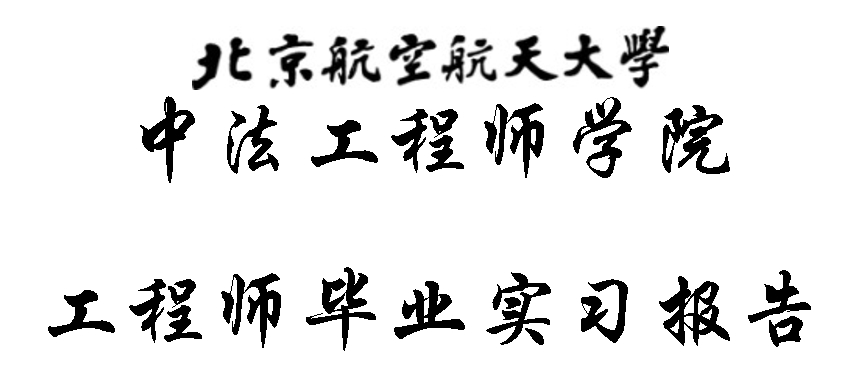
\includegraphics[width=.5\textwidth]{pic/head-intern}
  \bicaption{测试图片\\第二行题注}{Test Pic\\Sec Row}
  \label{fig:logo}
\end{figure}

\section{数学环境}

\subsection{数学符号}

模板定义了一些正体(upright)的数学符号:
\begin{center}
  \begin{tabular}{rl}
    \toprule
    符号                 & 命令 \\
    \midrule
    常数$\eu$     & \verb|\eu| \\
    复数单位$\iu$ & \verb|\iu| \\
    微分符号$\diff$ & \verb|\diff| \\
    $\argmax$         & \verb|\argmax| \\
    $\argmin$         & \verb|\argmin| \\
    \bottomrule
  \end{tabular}
\end{center}

更多的例子:
\begin{equation}
\eu^{\iu\pi} + 1 = 0
\end{equation}
\begin{equation}
\frac{\diff^2u}{\diff t^2} = \int f(x) \diff x
\end{equation}
\begin{equation}
\argmin_x f(x)
\end{equation}

\subsection{定理、引理和证明}

\begin{definition}
  If the integral of function $f$ is measurable and non-negative, we define
  its (extended) \textbf{Lebesgue integral} by
  \begin{equation}
  \int f = \sup_g \int g,
  \end{equation}
  where the supremum is taken over all measurable functions $g$ such that
  $0 \leq g \leq f$, and where $g$ is bounded and supported on a set of
  finite measure.
\end{definition}

\begin{example}
  Simple examples of functions on $\mathbf{R}^d$ that are integrable
  (or non-integrable) are given by
  \begin{equation}
  f_a(x) =
  \begin{cases}
  |x|^{-a} & \text{if } |x| \leq 1,\\
  0 & \text{if } x > 1.
  \end{cases}
  \end{equation}
  \begin{equation}
  F_a(x) = \frac{1}{1 + |x|^a}, \qquad \text{all } x \in \mathbf{R}^d.
  \end{equation}
  Then $f_a$ is integrable exactly when $a < d$, while $F_a$ is integrable
  exactly when $a > d$.
\end{example}

\begin{lemma}[Fatou]
  Suppose $\{f_n\}$ is a sequence of measurable functions with $f_n \geq 0$.
  If $\lim_{n \to \infty} f_n(x) = f(x)$ for a.e. $x$, then
  \begin{equation}
  \int f \leq \liminf_{n \to \infty} \int f_n.
  \end{equation}
\end{lemma}

\begin{remark}
  We do not exclude the cases $\int f = \infty$,
  or $\liminf_{n \to \infty} f_n = \infty$.
\end{remark}

\begin{corollary}
  Suppose $f$ is a non-negative measurable function, and $\{f_n\}$ a sequence
  of non-negative measurable functions with
  $f_n(x) \leq f(x)$ and $f_n(x) \to f(x)$ for almost every $x$. Then
  \begin{equation}
  \lim_{n \to \infty} \int f_n = \int f.
  \end{equation}
\end{corollary}

\begin{proposition}
  Suppose $f$ is integrable on $\mathbf{R}^d$. Then for every $\epsilon > 0$:
  \begin{enumerate}
    \renewcommand{\theenumi}{\roman{enumi}}
    \item There exists a set of finite measure $B$ (a ball, for example) such that
    \begin{equation}
    \int_{B^c} |f| < \epsilon.
    \end{equation}
    \item There is a $\delta > 0$ such that
    \begin{equation}
    \int_E |f| < \epsilon \qquad \text{whenever } m(E) < \delta.
    \end{equation}
  \end{enumerate}
\end{proposition}

\begin{theorem}
  Suppose $\{f_n\}$ is a sequence of measurable functions such that
  $f_n(x) \to f(x)$ a.e. $x$, as $n$ tends to infinity.
  If $|f_n(x)| \leq g(x)$, where $g$ is integrable, then
  \begin{equation}
  \int |f_n - f| \to 0 \qquad \text{as } n \to \infty,
  \end{equation}
  and consequently
  \begin{equation}
  \int f_n \to \int f \qquad \text{as } n \to \infty.
  \end{equation}
\end{theorem}

\begin{proof}
  Trivial.
\end{proof}



\subsection{自定义}

\newtheorem*{axiomofchoice}{Axiom of choice}
\begin{axiomofchoice}
  Suppose $E$ is a set and ${E_\alpha}$ is a collection of
  non-empty subsets of $E$. Then there is a function $\alpha
  \mapsto x_\alpha$ (a ``choice function'') such that
  \begin{equation}
  x_\alpha \in E_\alpha,\qquad \text{for all }\alpha.
  \end{equation}
\end{axiomofchoice}

\newtheorem{observation}{Observation}[chapter]
\begin{observation}
  Suppose a partially ordered set $P$ has the property
  that every chain has an upper bound in $P$. Then the
  set $P$ contains at least one maximal element.
\end{observation}
\begin{proof}[A concise proof]
  Obvious.
\end{proof}

\newtheorem{observationvar2}[observation]{Observationvar2}
\begin{observationvar2}
  Suppose a partially ordered set $P$ has the property
  that every chain has an upper bound in $P$. Then the
  set $P$ contains at least one maximal element.
\end{observationvar2}
\begin{proof}[A concise proof]
  Obvious.
\end{proof}


%-----------------------------
\section{宏包使用}

请将以下文件与此LaTeX文件放在同一目录中:

\begin{tabular}{ll}
 \verb|ecpknstage.cls |                 & $\triangleright$ LaTeX宏模板文件 \\
 \verb|bst/GBT7714-BUAA.bst|      & $\triangleright$ 国标参考文献BibTeX样式文件2015 \\
 \verb|pic/head-intern.eps|         & $\triangleright$ 论文封皮 \\
 \verb|tex/*.tex|                 & $\triangleright$ 本模板样例中的独立章节\\
\end{tabular}\\

通过 \verb|\documentclass[| \verb|<printtype>,| \verb|<ostype>,| \verb|<ctexbookoptions>| \verb|]{EcpknStage}|载入宏包:
\begin{itemize}
  \item[{\tt printtype} $\triangleright$] 打印设置(printtype),可选值: \\
    a) 单面打印(\verb|oneside|)[缺省值]\\
    b) 双面打印(\verb|twoside|)
  \item[{\tt ostype} $\triangleright$] 系统类型(printtype),可选值: \\
    a) Windows(\verb|win|)[缺省值]\\
    b) Linux(\verb|linux|)\\
    c) Mac(\verb|mac|)
  \item[{\tt ctexbookoptions} $\triangleright$] {\tt ctexbook}文档类支持的其他选项: \\
    使用{\tt ctexbookoptions}选项传递{\tt ctexbook}文档类支持的其他选项。
    例如,使用{\tt fontset=founder}选项启用方正字体以避免生僻字乱码的问题\footnote{需要系统安装方正字体。}。
\end{itemize}


\setlength{\hangindent}{4em}
模板已内嵌LaTeX工具包:\\
{\tt ifthen},{\tt etoolbox},{\tt titletoc},{\tt remreset},
{\tt geometry},{\tt fancyhdr},{\tt setspace},{\tt float},
{\tt graphicx},{\tt subfigure},{\tt epstopdf},{\tt array},{\tt enumitem},
{\tt booktabs},{\tt longtable},{\tt multirow},{\tt caption},
{\tt listings},{\tt algorithm2e},{\tt amsmath},{\tt amsthm},
{\tt hyperref},{\tt pifont},{\tt color},{\tt soul};\\
For Windows: {\tt times}, {\tt newtxmath};\\
For Linux: {\tt newtxtext}, {\tt newtxmath};\\
For Mac: {\tt times}, {\tt fontspec}。


模板已内嵌宏:\verb|\highlight{text}|(黄色高亮)。

请统一使用UTF-8编码。



%-----------------------------
\section{选项设置}

\begin{itemize}[leftmargin=3cm]
  \item[{\tt  $\backslash$refcolor} $\triangleright$]  开启/关闭引用编号颜色,包括参考文献,公式,图,表,算法等\\
  \texttt{on}:开启 [默认]\\
  \texttt{off}:关闭
  \item[{\tt $\backslash$beginright} $\triangleright$]  摘要和正文从右侧页开始\\
  \texttt{on}:开启 [默认]\\
  \texttt{off}:关闭
  \item[{\tt $\backslash$emptypageword} $\triangleright$]  空白页留字
  \item[{\tt $\backslash$Listfigtab} $\triangleright$]  是否使用图标清单目录\\
  \texttt{on}:开启 [默认]\\
  \texttt{bi}:双标题\\
  \texttt{off}:关闭
\end{itemize}


%-----------------------------
\section{章节撰写}
本模板支持以下标题级别标题级别:

\begin{tabular}{ll}
  \verb|\chapter{章}|              & $\triangleright$ 第一章 \\
  \verb|\chapter*{无章号章}|       & $\triangleright$ 无章号章 \\
  \verb|\chaptera{无章号有目录章}| & $\triangleright$ 无章号有目录章 \\
  \verb|\summary|                  & $\triangleright$ 总结\\
  \verb|\appendix|                 & $\triangleright$ 附录\\
  \verb|\multappendix|             & $\triangleright$ 多附录\\
  \verb|\achievement|              & $\triangleright$ 攻读学位期间取得的成果\\
  \verb|\acknowledgments|          & $\triangleright$ 致谢\\
  \verb|\biography|                & $\triangleright$ 作者简介\\
  \verb|\section{节}|              & $\triangleright$ 1.1 节\\
  \verb|\subsection{条}|           & $\triangleright$ 1.1.1 条\\
  \verb|\subsubsection{A}|         & $\triangleright$ 1.1.1.1 A\\
  \verb|\paragraph{a}|             & $\triangleright$ 1.1.1.1.1 a\\
  \verb|\subparagraph{a)}|         & $\triangleright$ 1.1.1.1.1.1 a)\\
\end{tabular}

%-----------------------------
\section{注意事项}
\begin{itemize}
  \item[$\triangleright$] \textit{中文斜体}将转换为楷体;
  \item[$\triangleright$] \textbf{中文粗体}在Windows(From WeiQM)和Mac(From CaiBW)下转换为黑体,Linux下正常(From QiaoJF);
  \item[$\triangleright$] \verb|\label{<text>}|中不能使用中文;
  \item[$\triangleright$] 浮动体与正文之间的距离是弹性的,根据内容调整,不太好控制;
  \item[$\triangleright$] 命令符与汉字之间请注意加空格以避免undefined错误(pdfLaTeX下好像一般不存在这个问题,主要在XeLaTeX编译环境下发生);
\end{itemize}

%-----------------------------
\section{意见及问题反馈}
\indent GitHub:\href{https://github.com/lcs27/ECPKNStage/issues}{https://github.com/lcs27/ECPKNStage/issues}

\input{tex/chap_acknowledge}

\end{document}
